\documentclass[xelatex,ja=standard,a4paper,14pt,everyparhook=compat]{bxjsarticle}
\usepackage{amsmath, amssymb, amsthm}
\usepackage{mathtools, bm}
\usepackage{enumitem}
\setenumerate{label=\alph*.}

% \usepackage{concmath}
% \usepackage[OT1]{fontenc}
% \setsansfont{Computer Mathematics}
% \setmainfont{CMU Concrete}
% \setCJKmainfont{Noto Sans JP Light}
% \setCJKsansfont{Noto Sans JP Light}

\usepackage{fancyhdr}
\pagestyle{fancy}
\rhead{\leftmark}
\lhead{\rightmark}
\renewcommand{\footrulewidth}{0.4pt}
\let\origtitle\title
\renewcommand{\title}[1]{\lfoot{#1}\origtitle{#1}}
\cfoot{}
\rfoot{\thepage}

\newcommand{\paren}[1]{\left(#1\right)}

\newcommand{\bbC}{\mathbb{C}}
\newcommand{\bbN}{\mathbb{N}}
\newcommand{\bbP}{\mathbb{P}}
\newcommand{\bbF}{\mathbb{F}}
\newcommand{\frakS}{\mathfrak{S}}
\DeclareMathOperator{\inv}{inv}
\DeclareMathOperator{\conv}{conv}
\DeclareMathOperator{\image}{Im}

\theoremstyle{definition}
\newtheorem{theorem}{定理}
\newtheorem*{theorem*}{定理}
\newtheorem{lemma}{補題}
\newtheorem*{lemma*}{補題}
\newtheorem{example}[theorem]{例}
\newtheorem*{example*}{例}
\newtheorem{definition}[theorem]{定義}
\newtheorem*{definition*}{定義}
\newtheorem{proposition}[theorem]{命題}
\newtheorem*{proposition*}{命題}
\newtheorem{corollary}[theorem]{系}
\newtheorem{problem}{問題}
\newtheorem*{answer}{解答}
\renewcommand{\proofname}{\textup{証明}}

\usepackage{tcolorbox}
\tcbuselibrary{breakable,skins,theorems}

\tcolorboxenvironment{definition}{
    coltitle = black,
    % colback = white,
    colframe = green!35!black,
    fonttitle = \bfseries,
    breakable = true
}

\tcolorboxenvironment{definition*}{
    coltitle = black,
    % colback = white,
    colframe = green!35!black,
    fonttitle = \bfseries,
    breakable = true
}

\tcolorboxenvironment{theorem}{
    coltitle = black,
    % colback = black!10!white,
    colframe = blue!35!black,
    fonttitle = \bfseries,
    breakable = true
}

\tcolorboxenvironment{theorem*}{
    coltitle = black,
    % colback = black!10!white,
    colframe = blue!35!black,
    fonttitle = \bfseries,
    breakable = true
}

\tcolorboxenvironment{proposition}{
    coltitle = black,
    % colback = black!10!white,
    colframe = green!35!black,
    fonttitle = \bfseries,
    breakable = true
}

\tcolorboxenvironment{proposition*}{
    coltitle = black,
    % colback = black!10!white,
    colframe = green!35!black,
    fonttitle = \bfseries,
    breakable = true
}

\tcolorboxenvironment{lemma}{
    coltitle = black,
    % colback = black!10!white,
    colframe = gray!35!black,
    fonttitle = \bfseries,
    breakable = true
}

\tcolorboxenvironment{example}{
    coltitle = black,
    % colback = black!10!white,
    colframe = purple!35!black,
    fonttitle = \bfseries,
    breakable = true
}

\tcolorboxenvironment{example*}{
    coltitle = black,
    % colback = black!10!white,
    colframe = purple!35!black,
    fonttitle = \bfseries,
    breakable = true
}

\tcolorboxenvironment{lemma*}{
    coltitle = black,
    % colback = black!10!white,
    colframe = gray!35!black,
    fonttitle = \bfseries,
    breakable = true
}

\tcolorboxenvironment{proof}{
    blanker,
    breakable,
    left=5mm,
    before skip=10pt,
    after skip=10pt,
    borderline west={1mm}{0pt}{black}
}

\tcolorboxenvironment{proof*}{
    blanker,
    breakable,
    left=5mm,
    before skip=10pt,
    after skip=10pt,
    borderline west={1mm}{0pt}{black}
}

\tcolorboxenvironment{problem}{
    coltitle = black,
    % colback = black!10!white,
    colframe = black!35!black,
    fonttitle = \bfseries,
    breakable = true
}

\tcolorboxenvironment{answer}{
    blanker,
    breakable,
    left=5mm,
    before skip=10pt,
    after skip=10pt,
    borderline west={1mm}{0pt}{black}
}

\title{3.5 Chains in Distributive Lattices \\ 3.6 Incidence Algebras}
\author{shino16}
\date{\today}

\begin{document}

\begin{titlepage}
    \maketitle
    \tableofcontents
\end{titlepage}

\setcounter{section}{-1}
\section{復習}

\begin{proposition*}[3.5.1]
    有限半順序集合$P$,$m \in \bbN$について以下は全て等しい: \begin{enumerate}
        \item 順序を保つ$\sigma: P \to \bm{m}$の写像の個数,
        \item $J(P)$における長さ$m$の多重鎖$\hat 0 = I_0 \leq I_1 \leq \cdots \leq I_m = \hat 1$の個数.
        \item $J(P \times \bm{m-1})$の位数.
    \end{enumerate}
\end{proposition*}
\begin{figure}[h]
    \centering
    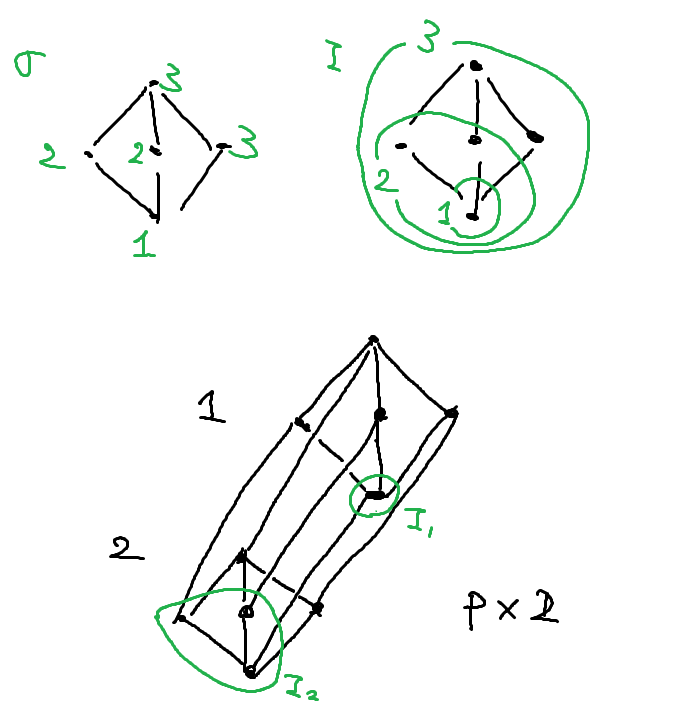
\includegraphics[width=0.7  \textwidth]{Prop3.5.1.png}
    \caption{$P = \Pi_3$,$m = 3$の例}
\end{figure}

\newpage

\begin{proposition}[3.5.2] \label{3.5.2}
    有限半順序集合$P$,$m \in \bbN$について以下は等しい: \begin{enumerate}
        \item 順序を保つ全射$\sigma: P \to \bm{m}$の写像の個数,
        \item $J(P)$における長さ$m$の鎖$\hat 0 = I_0 < I_1 < \cdots < I_m = \hat 1$の個数.
    \end{enumerate}
\end{proposition}

\section{線形順序拡大}

\begin{definition*}
    $\#P = p$のとき,順序を保つ全単射$\sigma: P \to \bm{p}$を\textbf{線形順序拡大(linear extension)}または\textbf{トポロジカルソート}といい,線形順序拡大の個数を$e(P)$で表す.
\end{definition*}

\subsection{格子パスとの対応}

命題\ref{3.5.2}より, \begin{align*}
    e(P) & = (\text{$J(P)$上の鎖$\hat 0 = I_0 < I_1 < \cdots < I_{\#P} = \hat 1$の個数}) \\
         & = (\text{$J(P)$上の極大なパスの個数}).
\end{align*}
そこで,$J(P)$上の鎖をある種の格子上のパスと対応付ける.

$P$の鎖への分割$C_1,\ldots,C_k$をとる.$\delta: J(P) \to \bbN^k$を \begin{equation*}
    \delta(I) = (\#(I \cap C_1), \#(I \cap C_2), \ldots, \#(I \cap C_k))
\end{equation*}
で定める.

\newpage

\begin{lemma*}
    $\bbN^k$を辞書式順序のもとで半順序集合(特に束)とみなすとき,$\delta$は \begin{enumerate}
        \item 単射,
        \item 束同士の準同型写像,
              % \item ランクを保つ,
        \item $J(P) \cong \image \delta$.
    \end{enumerate}
    したがって$J(P)$上の極大なパスは$\image \delta$における格子パスと一対一に対応する.
\end{lemma*}
\begin{proof}
    \begin{enumerate}
        \item 順序イデアル$I \in J(P)$は,$I$の極大元の集合で特徴づけられる.各鎖は$I$の極大元を高々$1$個しか含まないので,極大元の集合が異なれば$\delta$の像も異なる.
        \item $I_1 \lor I_2 = I_1 \cup I_2$,$I_1 \land I_2 = I_1 \cap I_2$に注意.$\bbN^k$上では$\lor$は各点$\max$,$\land$は各点$\min$.

              鎖$C_i$について, \begin{align*}
                  \#((I_1 \cup I_2) \cap C_i) & = \max(\#(I_1 \cap C_i), \#(I_2 \cap C_i)), \\
                  \#((I_1 \cap I_2) \cap C_i) & = \min(\#(I_1 \cap C_i), \#(I_2 \cap C_i)).
              \end{align*}
              % \item $I \in J(P)$のランクは$\#I$,$\delta(I) \in \bbN^k$のランクは$\sum_i \#(I \cap C_i) = \#I$.
        \item $I_1, I_2 \in J(P)$について, \begin{align*}
                  I_1 \leq I_2
                   & \Longleftrightarrow I_1 \land I_2 = I_1                                                   \\
                   & \Longleftrightarrow \delta(I_1 \land I_2) = \delta(I_1)         &  & (\because \text{a.}) \\
                   & \Longleftrightarrow \delta(I_1) \land \delta(I_2) = \delta(I_1) &  & (\because \text{b.}) \\
                   & \Longleftrightarrow \delta(I_1) \leq \delta(I_2),
              \end{align*}
    \end{enumerate}
\end{proof}

\subsection{具体例}

\begin{figure}[ht]
    \centering
    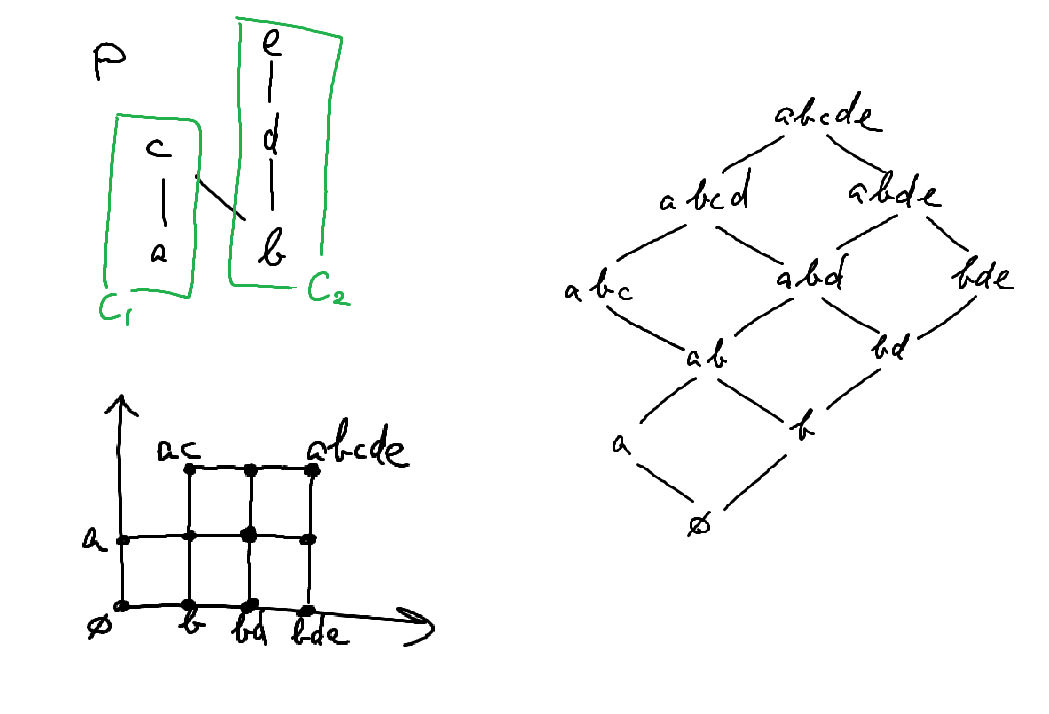
\includegraphics[width=0.9\textwidth]{gamma.png}
    \caption{例3.5.3}
\end{figure}

\begin{example*}[3.5.4]
    位数$m,n$の鎖$C_1,C_2$をとり,$P = C_1 + C_2$とする.

    このとき$\image \delta \cong \bm{m} \times \bm{n}$.したがって$e(P) = \binom{m+n}{m}$.

    より一般に,$P = P_1 + \cdots + P_k$,$n_i = \#P_i$とすると, \begin{equation*}
        e(P) = \binom{n_1+\cdots+n_k}{n_1,\ldots,n_k} e(P_1) e(P_2) \cdots e(P_k).
    \end{equation*}
\end{example*}

\begin{example*}[3.5.5]
    $P = \bm{2} \times \bm{n}$,$C_1 = \{(2,j) : j \in \bm{n}\}$,$C_2 = \{(1,j):j \in \bm{n}\}$とする.

    このとき$\image \delta = \{(i,j) : 0 \leq i \leq j \leq n\}$.この上での格子パスの個数はカタラン数$C_n = \frac{1}{n+1}\binom{2n}{n}$.
\end{example*}
\begin{figure}[ht]
    \centering
    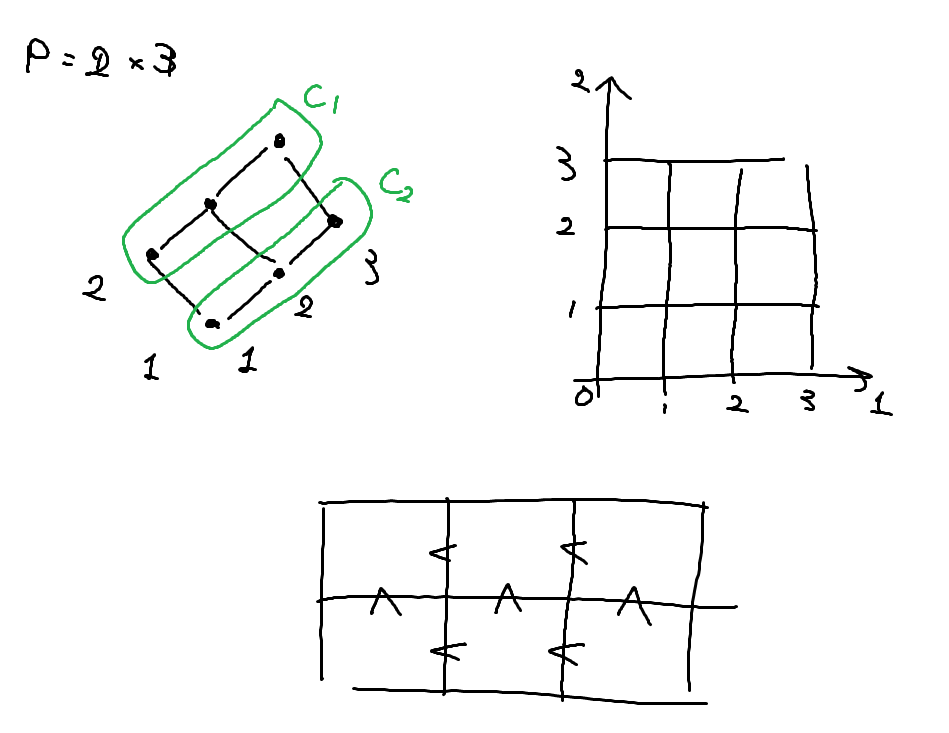
\includegraphics[width=0.8\textwidth]{Fig3.11.png}
    \caption{$P = \bm2 \times \bm3$とstandard Young tableauの例}
\end{figure}

\subsection{パスカルの三角形との関係}

各$I \in J(P)$について,$I$を半順序集合とみなしたときの線形順序拡大の個数を$e(I)$とする.$I$のトポロジカルソートを最後の点で分けて数えると, \begin{equation*}
    e(I) = \sum_{\substack{I' \in J(P) \\ I' \lessdot I}} e(I').
\end{equation*}

\begin{example*}
    $P = \bbN + \bbN$とし,$P$の有限順序イデアルの集合を$J_f(P)$とする.

    このとき$J_f(P) \cong \bbN \times \bbN$.

    $J_f(P)$のハッセ図において各$I \in J_f(P)$を$e(I)$でラベル付けすると,パスカルの三角形が得られる.
\end{example*}

\begin{definition*}
    有限的分配束$L = J_f(P)$と,対応する$e:L \to \bbP$をあわせて\textbf{一般パスカル三角形}と呼ぶ.
\end{definition*}

% ここで \begin{equation*}
%     \Gamma_\delta = \bigcup_{\substack{[I_1,I_2] \subseteq J(P) \\ \text{ブール代数}}} \conv(\delta([I_1,I_2]))
% \end{equation*}
% を考える ($\conv(\bullet)$は凸包を表す).
% \begin{figure}[h]
%     \centering
%     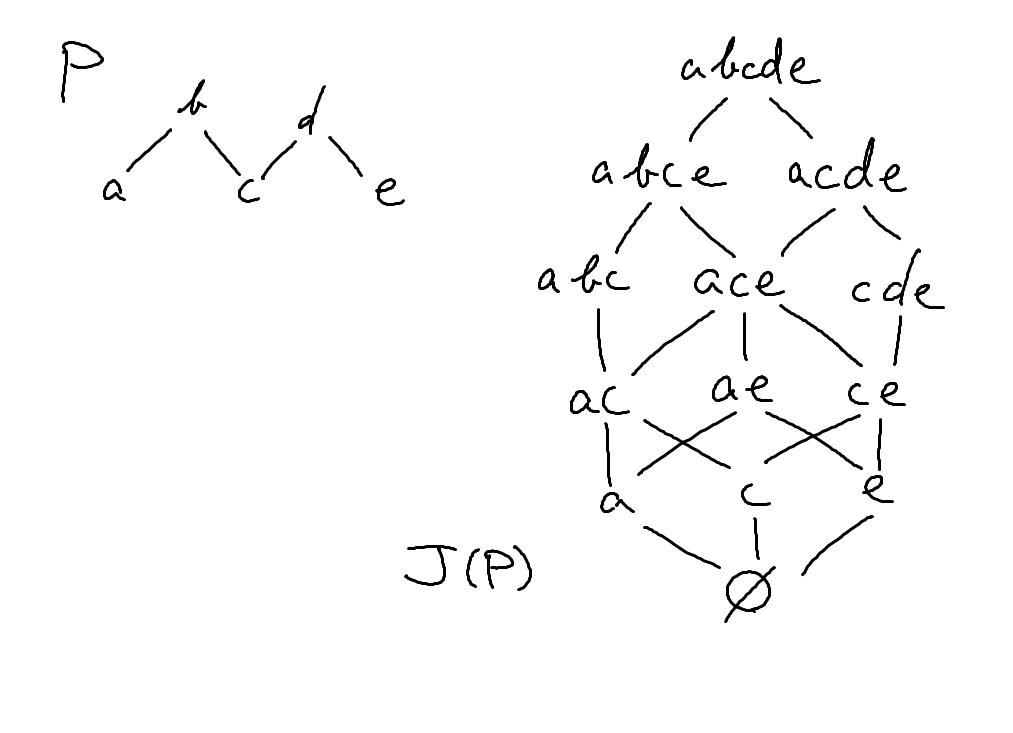
\includegraphics[width=0.8\textwidth]{J(P).png}
% \end{figure}

% \begin{proposition}
%     \begin{enumerate}
%         \item $[I_1,I_2] \subseteq J(P)$がブール代数と同型であるとき,$\conv(\delta([I_1,I_2]))$は$\ell(I_1,I_2)$次元の単位立方体.
%         \item $J(P)$上の極大な鎖は,$\Gamma_\delta$内の$\delta(\hat 0)$から$\delta(\hat 1)$への格子上のパスと一対一に対応する.
%     \end{enumerate}
% \end{proposition}
% \begin{proof}
%     \begin{enumerate}
%         \item $I_2 = I_1 \cup \{t_1,\ldots, t_k\}$とおく.各$i$について$I_1 \cup \{t_i\} \in J(P)$より,$t_1,\ldots,t_k$のうち$2$つが同じ鎖$C_j$に属することはない.
%     \end{enumerate}
% \end{proof}



% \newpage

% \section{演習問題}

% \setcounter{problem}{14}
% \begin{problem}
%     実数の閉区間に対して順序を$[a,b] < [c,d]$ iff $b < c$で定めるとき,実数の閉区間の集合と同型な半順序集合を\textbf{区間順序}という. \begin{enumerate}
%         \item 次を示せ: \begin{align*}
%             &\text{$P$は区間順序} \\
%             &\text{$\Longleftrightarrow$ $P$は$\bm 2 + \bm 2$と同型な部分半順序集合を持たない}
%         \end{align*}
%     \end{enumerate}
% \end{problem}

% \setcounter{problem}{6}
% \begin{problem}
%     \begin{enumerate}
%         \item 有限半順序集合$P$について,長さを$\ell$とするとき \begin{itemize}
%             \item どの$t \in P$も長さ$\ell$の鎖に含まれ,かつ
%             \item 長さ$\ell$未満の極大な鎖を含む
%         \end{itemize}
%         ものを構成せよ.
%         \item ある有限半順序集合$P$が孤立点を持たず,長さが$\ell$であるとする.

%         任意の$s \lessdot t$について,$s,t$をともに含む長さ$\ell$の鎖が存在するとき,$P$の任意の極大な鎖が長さ$\ell$であることを示せ.
%     \end{enumerate}
% \end{problem}

% \begin{problem}
%     次の条件を満たす有限半順序集合$P$を構成せよ: \begin{enumerate}
%         \item $s \leq t$ $\Longleftrightarrow$ $f(s) \geq f(t)$を満たす全単射$f: P \to P$が存在する.
%         \item $\forall t \in P$ $f(f(t)) = t$を満たす全単射$f$が存在しない.
%     \end{enumerate}
% \end{problem}

% \setcounter{problem}{76}

% \begin{figure}[h]
%     \centering
%     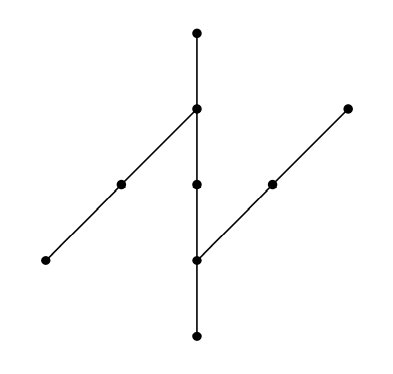
\includegraphics[width=0.3\textwidth]{Fig3.50.png}
%     \caption{例}
% \end{figure}

% \begin{problem}
% \begin{enumerate}
%     \item $p$元半順序集合$P$をとる.$i$個の鎖の和集合をとるとき,この位数の最大値が$\lambda_1 + \cdots + \lambda_i$と等しくなるように数列$(\lambda_i)$を定める.このとき$(\lambda_i)$が広義単調減少であることを示せ.
%     \item
% \end{enumerate}
% \end{problem}

\end{document}
